% \documentclass[aspectratio=169,notes]{beamer}
\documentclass[aspectratio=169]{beamer}
\usetheme[faculty=phil]{fibeamer}
\usepackage{polyglossia}
\setmainlanguage{english} %% main locale instead of `english`, you
%% can typeset the presentation in either Czech or Slovak,
%% respectively.
\setotherlanguages{russian} %% The additional keys allow
%%
%%   \begin{otherlanguage}{czech}   ... \end{otherlanguage}
%%   \begin{otherlanguage}{slovak}  ... \end{otherlanguage}
%%
%% These macros specify information about the presentation
\title[MaM]{Mechanics and Machines, Lecture 4} %% that will be typeset on the
\subtitle{Synthesis of planar mechanisms
\\ \        \\ \   
         } %% title page.
\author{Oleg Bulichev}
%% These additional packages are used within the document:
\usepackage{ragged2e}  % `\justifying` text
\usepackage{booktabs}  % Tables
\usepackage{tabularx}
\usepackage{tikz}      % Diagrams
\usetikzlibrary{calc, shapes, backgrounds}
\usetikzlibrary{decorations.pathreplacing,calligraphy,calc,graphs}
\usepackage{amsmath, amssymb}
\usepackage{url}       % `\url`s
\usepackage{listings}  % Code listings
% \usepackage{subfigure}
\usepackage{floatrow}
\usepackage{subcaption}
\usepackage{mathtools}
\usepackage{todonotes}
\usepackage{fontspec}
\usepackage{multicol}
\usepackage{pdfpages}
\usepackage{wrapfig}
\usepackage{animate}
\usepackage{booktabs}
\usepackage{multirow}
% \usepackage{graphicx}
\usepackage{colortbl}

\graphicspath{{resources/}}
\frenchspacing

\setbeamertemplate{caption}[numbered]
\usetikzlibrary{graphs}

% \usepackage[backend=biber,style=ieee,autocite=footnote]{biblatex}
% \addbibresource{biblio.bib}
% \DefineBibliographyStrings{english}{%
%   bibliography = {References},}

\newcommand{\oleg}[2][] {\todo[color=red, #1] {OLEG:\\ #2}}
\newcommand{\fbckg}[1]{\usebackgroundtemplate{\includegraphics[width=\paperwidth]{#1}}}%frame background

\usepackage[framemethod=TikZ]{mdframed}
\newcommand{\dbox}[1]{
\begin{mdframed}[roundcorner=3pt, backgroundcolor=yellow, linewidth=0]
\vspace{1mm}
{#1}
\vspace{1mm}
\end{mdframed}
}

\begin{document}
\setlength{\abovedisplayskip}{0pt}
\setlength{\belowdisplayskip}{0pt}
\setlength{\abovedisplayshortskip}{0pt}
\setlength{\belowdisplayshortskip}{0pt}

\fbckg{fibeamer/figs/title_page.png}
\frame[c]{\setcounter{framenumber}{0}
    \usebeamerfont{title}%
    \usebeamercolor[fg]{title}%
    \begin{minipage}[b][6.5\baselineskip][b]{\textwidth}%
        \textcolor{black}{\raggedright\inserttitle}
    \end{minipage}
    % \vskip-1.5\baselineskip

    \usebeamerfont{subtitle}%
    \usebeamercolor[fg]{framesubtitle}%
    \begin{minipage}[b][3\baselineskip][b]{\textwidth}
        \raggedright%
        \insertsubtitle%
    \end{minipage}
    \vskip.25\baselineskip
}
%   \frame[c]{\maketitle}

\fbckg{fibeamer/figs/common.png}

\note{\scriptsize \begin{itemize}
        \item \
    \end{itemize}}

\begin{frame}[c]{Difference between Analysis and Synthesis}
    \framesubtitle{}
    \vspace{-0.6cm}
    \begin{block}{Analysis}
        Analysis allows determining whether a given system will comply with certain requirements or not.

        During <<Theoretical Mechanics>> we only analyzed systems. We knew all dimensions and tried to find positions, velocities, accelerations.
    \end{block}

    \begin{block}{Synthesis}
        Synthesis is the design of a mechanism so that it complies with previously specified requirements.

        We know, that it should work on uneven terrain, and we are trying to design the robot with such possibilities. 
    \end{block}
\end{frame}

\begin{frame}[t]{Types of Synthesis}
\framesubtitle{}
\begin{columns}[T,onlytextwidth]
    \begin{column}{0.45\textwidth}
        \begin{exampleblock}{Structural}
            This synthesis deals with the \textbf{topological} and \textbf{structural study} of mechanisms. \smallskip
            
            It only considers the interconnectivity pattern of the links so that the results are unaffected by the changes in the geometric properties of the mechanisms.
        \end{exampleblock}
    \end{column}
    \begin{column}{0.45\textwidth}
        \begin{exampleblock}{Dimensional}
            It focuses on the problem of \textbf{obtaining the dimensions of a predefined mechanism} that has to comply with certain given requirements. \smallskip
            
            It will be necessary to define the dimension of the links and the position of the supports, among others.
        \end{exampleblock}
    \end{column}
\end{columns}
\end{frame}

\begin{frame}[t]{Structural Synthesis: Case Study}
    \framesubtitle{Structural synthesis problem}
    \only<1-2>{\large\begin{block}{Question}
            What the optimal number of legs should be in such robot mover?
        \end{block}}
    \only<2>{\large\begin{alertblock}{Answer}
            \centering Robot should have \textbf{8-14 legs} in total!
        \end{alertblock}}
\end{frame}

\begin{frame}[t]{Structural Synthesis: Case Study}
\framesubtitle{Criteria}
\vspace{-0.6cm}
\begin{figure}[H]
    \begin{minipage}{0.58\textwidth}
        \centering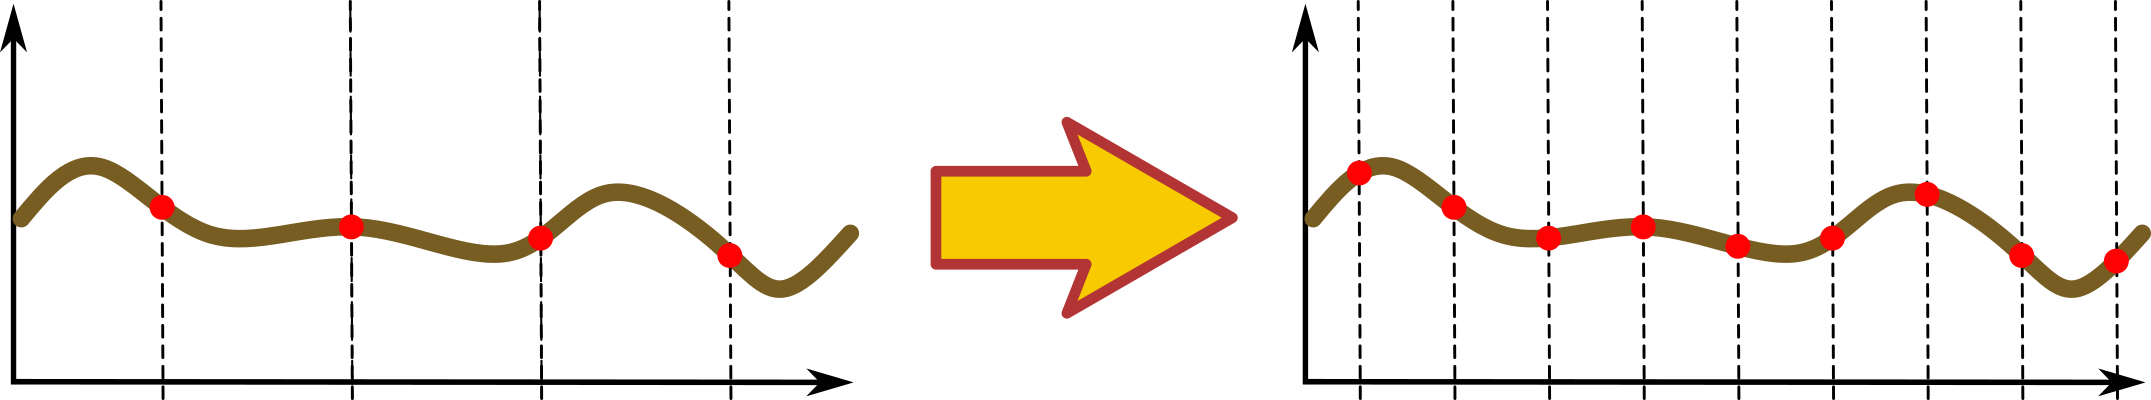
\includegraphics[height=2cm,width=1\textwidth,keepaspectratio]{f1.png}
    \end{minipage}\hfill
    \begin{minipage}{0.40\textwidth}
        More legs $\rightarrow$ higher data discretisation
        \label{fig:f1.png}
    \end{minipage}
\end{figure}
\vspace{-0.6cm}

\begin{figure}[H]
    \begin{minipage}{0.58\textwidth}
        \centering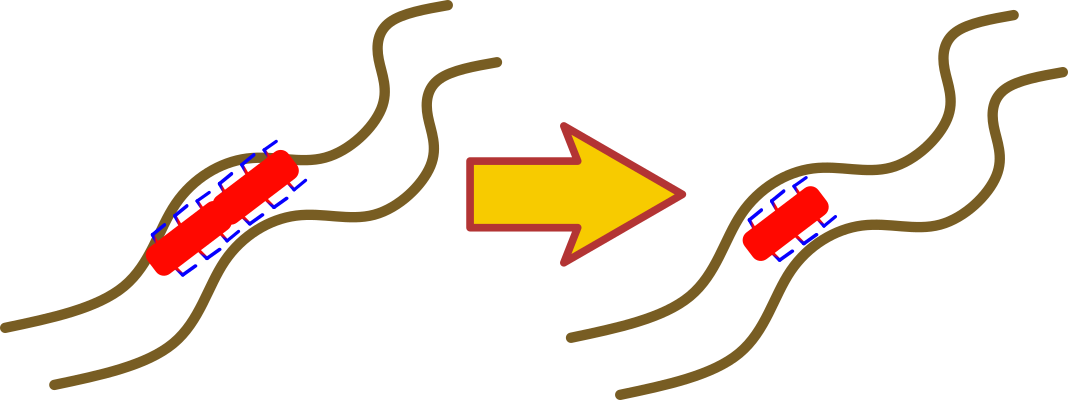
\includegraphics[height=2cm,width=1\textwidth,keepaspectratio]{f2.png}
    \end{minipage}\hfill
    \begin{minipage}{0.40\textwidth}
        More legs $\rightarrow$ longer robot $\rightarrow$ cannot pass though crooked terrains
        \label{fig:f2.png}
    \end{minipage}
\end{figure}
\vspace{-0.6cm}

\begin{figure}[H]
    \begin{minipage}{0.58\textwidth}
        \centering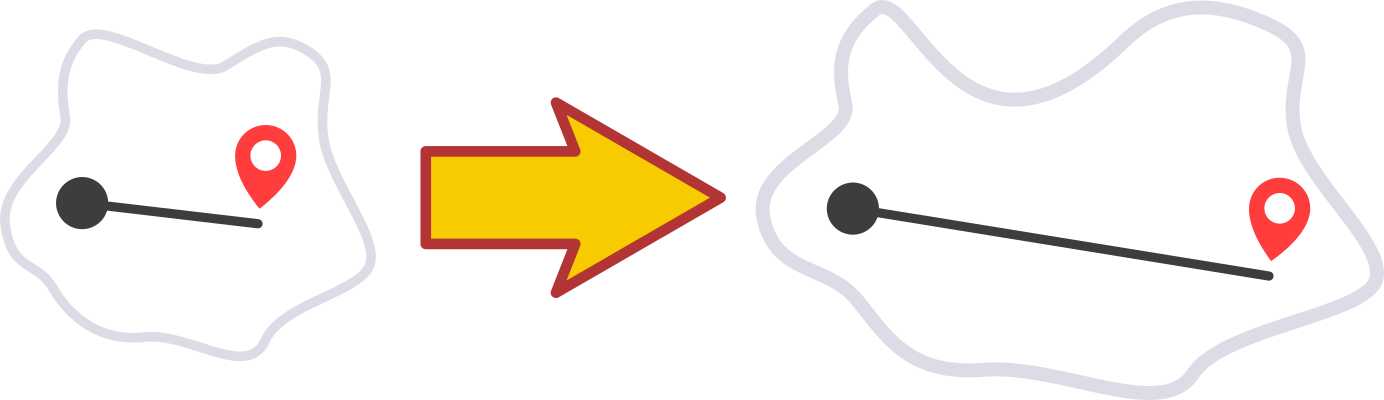
\includegraphics[height=2cm,width=1\textwidth,keepaspectratio]{f3.png}
    \end{minipage}\hfill
    \begin{minipage}{0.40\textwidth}
        Amount of legs nonlinearly correlates of maximal terrain passability
        \label{fig:f3.png}
    \end{minipage}
\end{figure}
\end{frame}

\begin{frame}[c]{Structural Synthesis: Case Study}
    \framesubtitle{Technological stack}
    \vspace{-0.9cm}
    \begin{figure}[H]
        \begin{subfigure}[t]{0.32\textwidth}
            \centering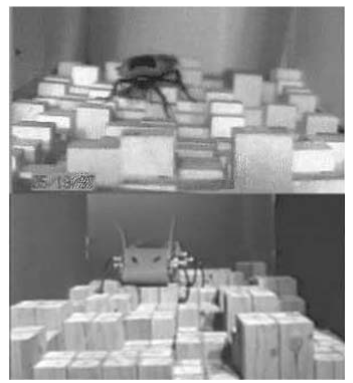
\includegraphics[height=4cm,width=1\textwidth,keepaspectratio]{c1_paper.png}
            \caption*{\small Generating terrain approach \\ (Robot traverse an \textbf{artificial terrain} based on \textbf{generating parameters})}
        \end{subfigure}
        \hfill
        \begin{subfigure}[t]{0.32\textwidth}
            \centering
\includegraphics[height=4cm,width=1\textwidth,keepaspectratio]{gazebo_logo.png}
            \caption*{Robot simulator}
        \end{subfigure}
        \hfill
        \begin{subfigure}[t]{0.32\textwidth}
            \centering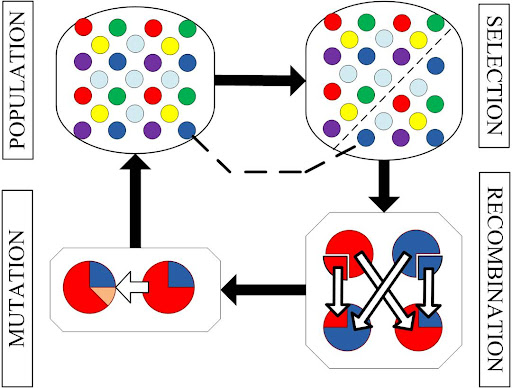
\includegraphics[height=5.5cm,width=1\textwidth,keepaspectratio]{gen_algo.jpg}
            \caption*{Genetic algorithm \\ (OpenAI-ES)}
        \end{subfigure}
        \hfill
    \end{figure}
\end{frame}

\begin{frame}[t]{Structural Synthesis: Case Study}
    \framesubtitle{Proposed solution}
    \begin{columns}[T,onlytextwidth]
        \begin{column}{0.49\textwidth}
            \begin{figure}[H]
                \centering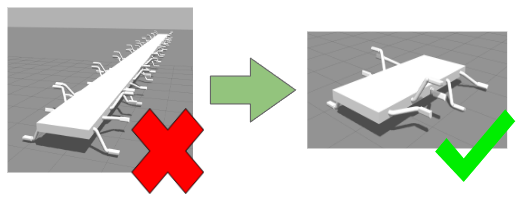
\includegraphics[height=3cm,width=1\textwidth,keepaspectratio]{optimization_idea.png}
                \caption*{\textbf{Idea}: Minimize number of legs without losing off-road passability}
                \label{fig{optimization_idea.png}}
            \end{figure}
        \end{column}
        \begin{column}{0.49\textwidth}
            \vspace{-2cm}
            \begin{figure}[H]
                \centering
                \begin{tikzpicture}
                    % Include the image in a node
                    \node [above right, inner sep=0] (image) at (0,0)
                    {\centering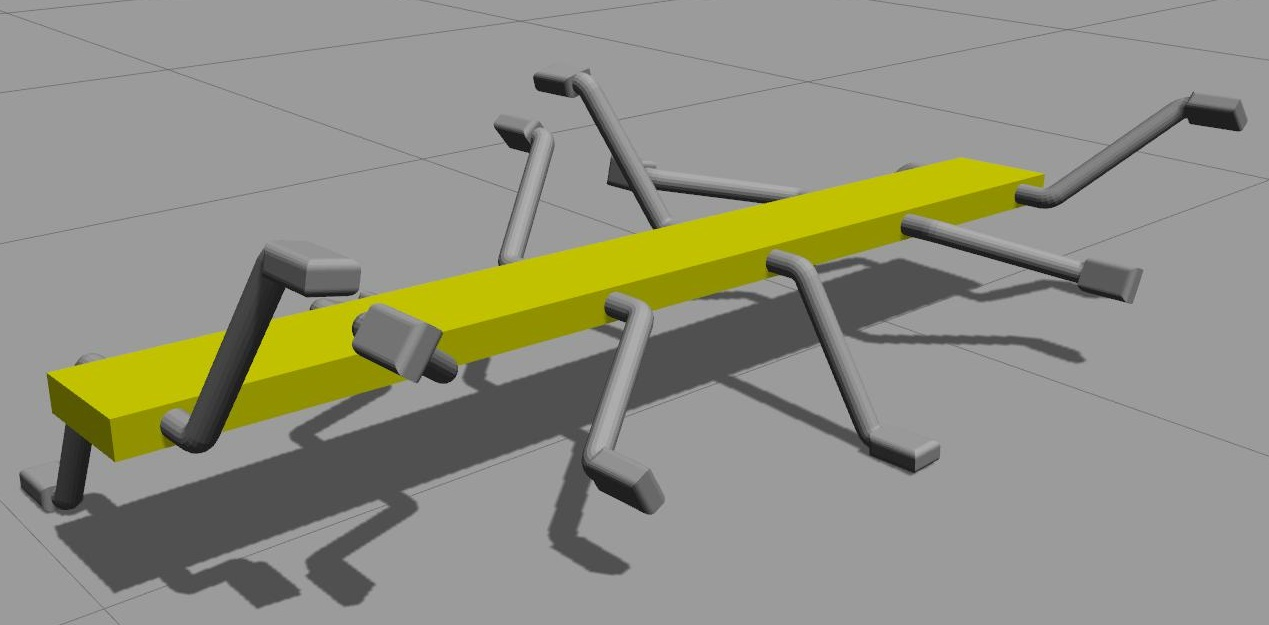
\includegraphics[height=2.5cm,width=1\textwidth,keepaspectratio]{best_gen_robot.jpg}};
                    % Create scope with normalized axes
                    \begin{scope}[
                            x={($ 0.1*(image.south east)$)},
                            y={($ 0.1*(image.north west)$)}]

                        % Labels
                        \draw [green, very thick,
                            decorate,
                            decoration = {brace,
                                    raise=5pt,
                                    amplitude=5pt,
                                    aspect=0.5}] (1.4,3.6) --  (8.1,6.8)
                        node[rounded corners=3pt, pos=0.5,above left =14pt,black,fill=white]{\tiny $(\gamma - 1) h_{\text{leg}}sin(\alpha)$};

                        \draw[stealth-, very thick,green] (9.5,7.8) -- (7.8,1.94);
                        \draw[stealth-, very thick,green] (1.5,2.8) -- (7,1)
                        node[rounded corners=3pt,right,black,fill=white]{\tiny $\gamma = 6$};

                        \draw[thin,green] (6.7,4) -- (5.75,9);
                        \draw[thin,green] (4.85,3.5) -- (5.75,9);
                        \draw[thin,green,stealth-stealth] (6.32,6) arc (-79.2:-99.2:3) node [rounded corners=3pt,below = 2pt,black,fill=white, midway] {\tiny $\alpha$};
                        % \draw[very thick,green] (8,6) -- (5,8);
                        % \draw[very thick,green] (0.5,2.5) rectangle (4.2,9)
                        % node[below left,black,fill=green]{\small test};
                    \end{scope}
                \end{tikzpicture}
                % \caption*{}
                \label{fig:best_gen_robot.jpg}
            \end{figure}
            \vspace{-1cm}
            {\footnotesize
                \begin{eqnarray*}
                    % \resizebox{0.9\hsize}{!}{
                    F \rightarrow max = \beta \left( {\omega}_{1} \cdot \overbrace{\delta}^{\text{Distance}} + {\omega}_{2} \cdot \overbrace{\frac{1}{(\gamma - 1) h_{\text{leg}}sin(\alpha)}}^{\text{Simplified body length}}\right) +\\ \nonumber + (1 - \beta) {\delta}^{{\omega}_{1}} {\left( \frac{1}{(\gamma - 1)h_{\text{leg}}sin(\alpha)}\right)}^{{\omega}_{2}}
                    % }
                \end{eqnarray*}
            }
            % \vspace{1pt}

            $\beta$ is adaptive parameter, \\ ${\omega}_{1,2} \in  [ 0..1 ] $ are the weight coefficients.
        \end{column}
    \end{columns}
\end{frame}

\begin{frame}[t]{Structural Synthesis: Case Study}
    \framesubtitle{Video: The story of one generated robot}
    \vspace{-0.6cm}
    \begin{figure}[H]
        % \href{run:./videos/pass_rand_terr.mp4}{
        \href{https://youtu.be/DcovvkTZgsg}{
            \centering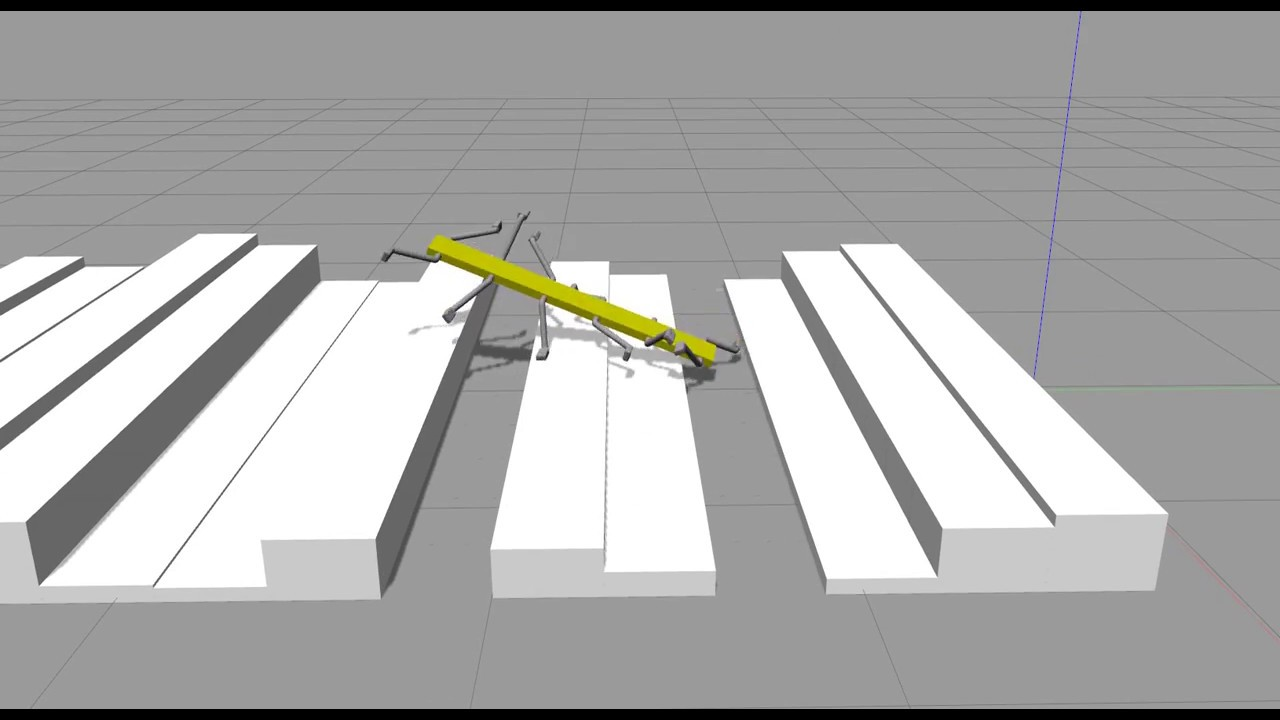
\includegraphics[height=6cm,width=1\textwidth,keepaspectratio]{genetic_video_preview.jpg}}
        % \caption{Click on a picture for a video}
    \end{figure}
\end{frame}

\begin{frame}[t]{Structural Synthesis: Case Study}
    \framesubtitle{Particular results: $\omega_1 = 0.6$, $\omega_2 = 0.4$}
    \vspace{-0.6cm}

    \begin{table}[H]
        \centering
        \begin{tabular}{c|c|c|c|c}
         & \textbf{\begin{tabular}[c]{@{}c@{}}Terrain\\ types\end{tabular}} & \textbf{No. Legs} & \textbf{\begin{tabular}[c]{@{}c@{}}Angle b/w\\ neighbor legs\end{tabular}} & \textbf{No. individuals} \\
         \hline
         \rule{0cm}{0.5cm}
        \textbf{Phase 1} &  & \cellcolor[HTML]{DAE8FC}12 & 73 & 200 \\ \cline{1-1} \cline{3-5} 
         & \multirow{-2}{*}{\begin{minipage}{2.5cm}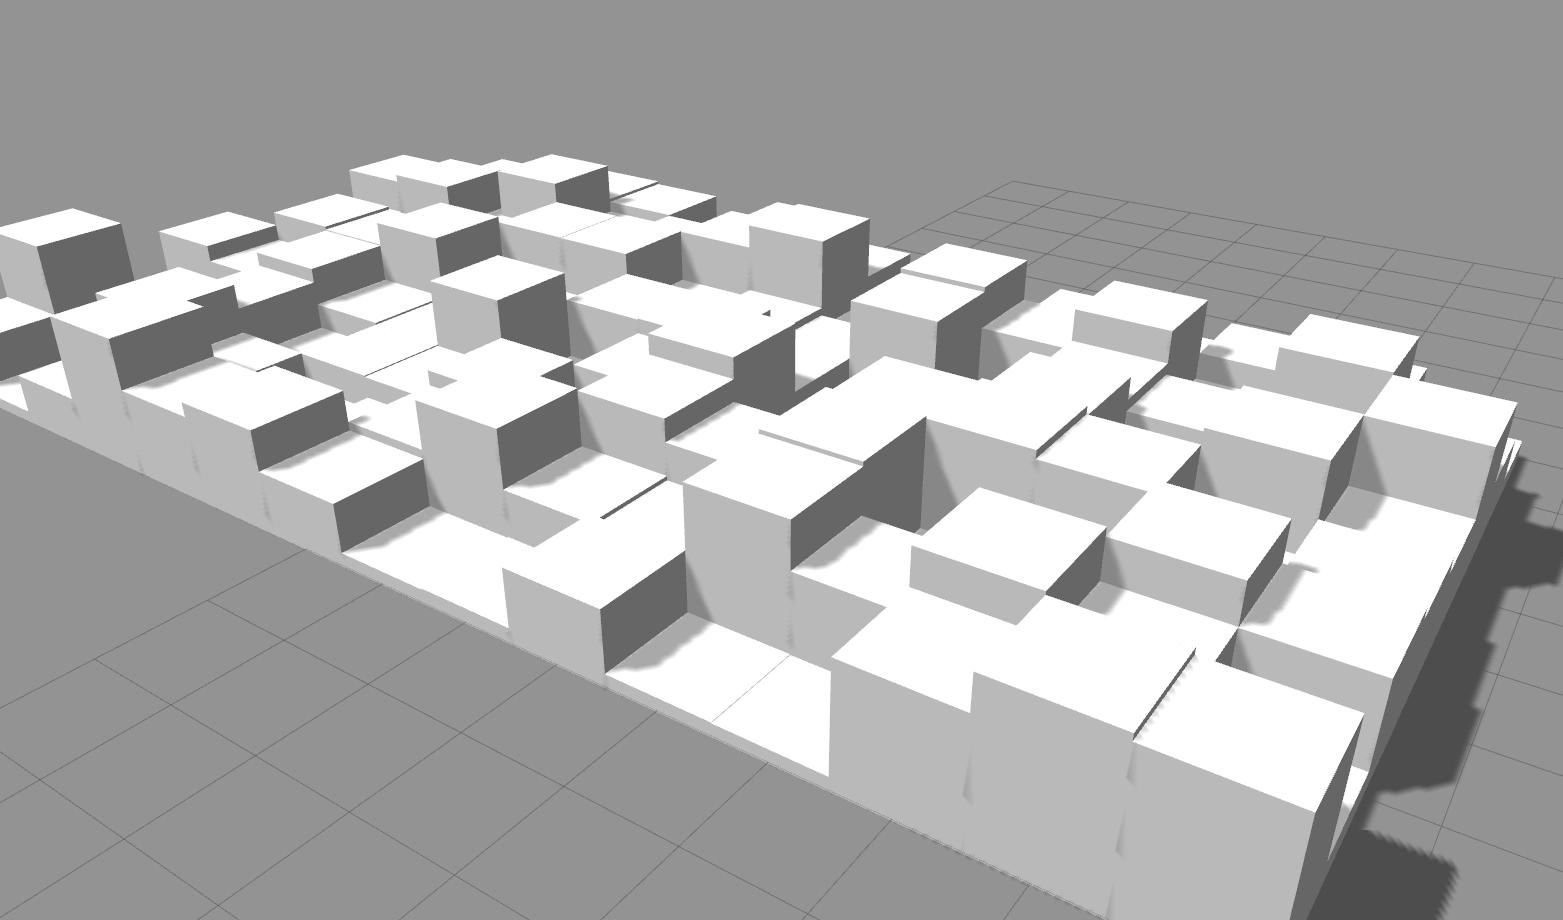
\includegraphics[height=3cm,width=2.5cm,keepaspectratio]{terrain_1.jpg}\end{minipage}} & \cellcolor[HTML]{DAE8FC}12 & 72 &  \\ [0.5cm] \cline{3-4} 
         & \begin{minipage}{2.5cm}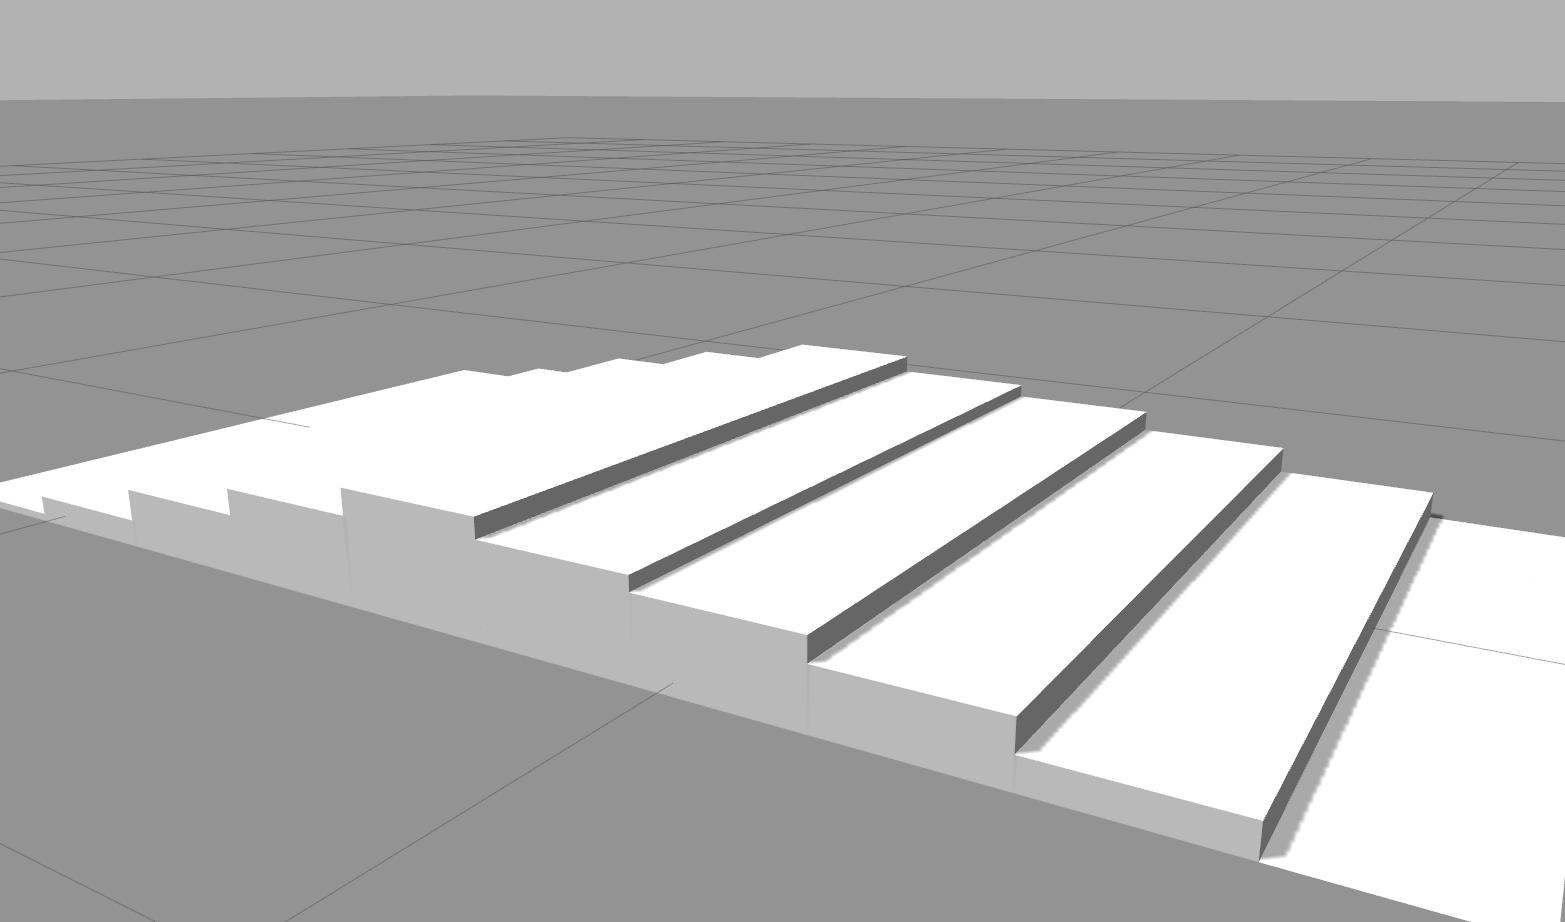
\includegraphics[height=3cm,width=2.5cm,keepaspectratio]{terrain_2.jpg}\end{minipage} & \cellcolor[HTML]{DAE8FC}10 & 68 &  \\ [0.5cm] \cline{3-4}
        \multirow{-3}{*}{\textbf{Phase 2}} & \begin{minipage}{2.5cm}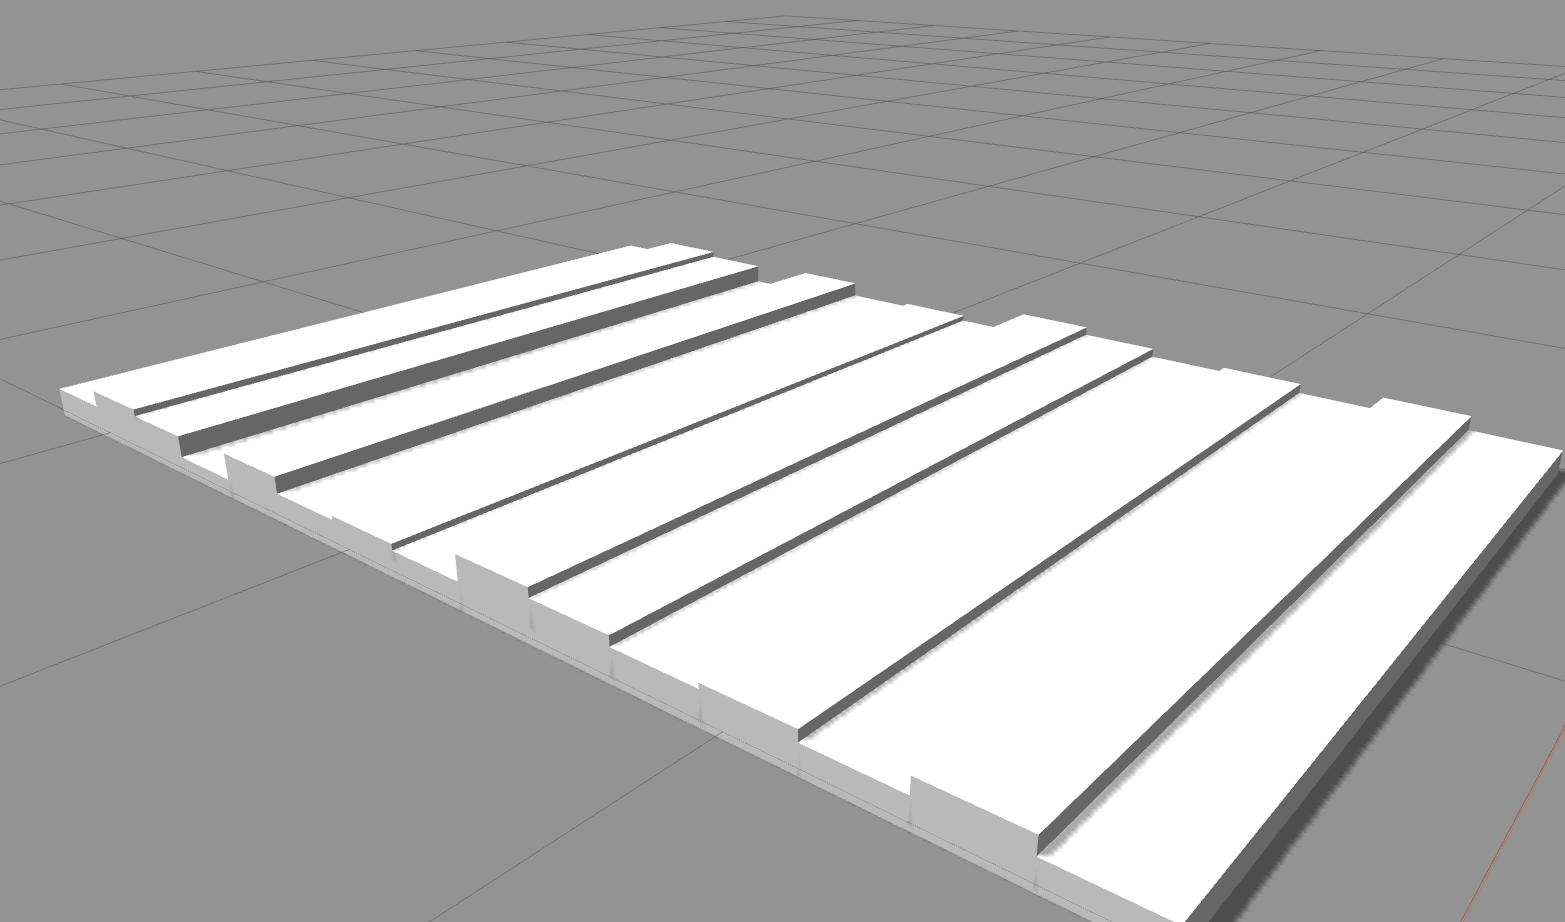
\includegraphics[height=3cm,width=2.5cm,keepaspectratio]{terrain_3.jpg}\end{minipage} & \cellcolor[HTML]{DAE8FC}12 & 77 & \multirow{-3}{*}{55}
        \end{tabular}
        % \caption*{\large\centering\textbf{Summary}: created robot should have 10-12 legs in total}
        \end{table}

\end{frame}

\begin{frame}[t]{Structural Synthesis: Case Study}
    \framesubtitle{Global results}
    \begin{columns}[T,onlytextwidth]
        \begin{column}{0.49\textwidth}
            Based on fitness function the number of legs range starts from 8 till 14 for different $\omega$ values. 
            
            It can be explained by static stability criteria. In such case 4 legs will touch the ground.    
        \end{column}
        \begin{column}{0.49\textwidth}
            \vspace{-1.5cm}
            \begin{figure}[H]
                \centering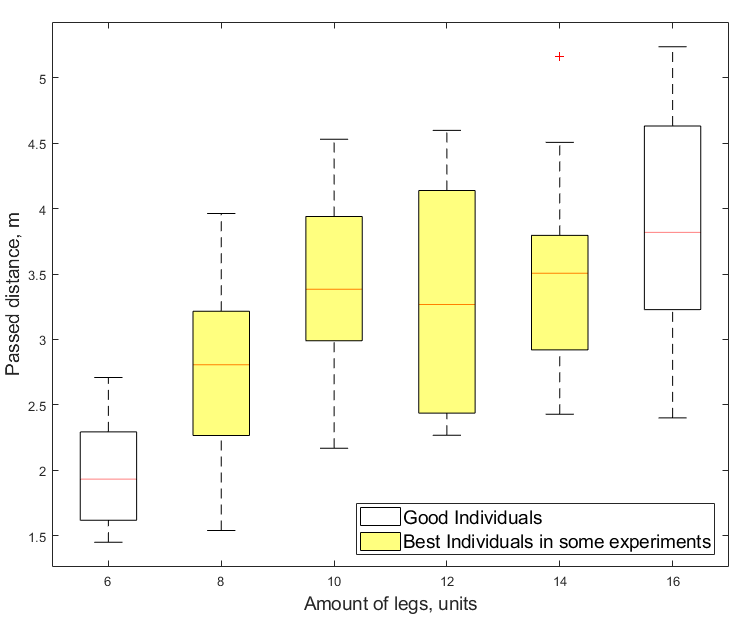
\includegraphics[height=5cm,width=1\textwidth,keepaspectratio]{box_plot_structural_synthesis.png}
                \caption*{Correlation between amount of legs and passed distance by best robot individuals from several experiments}
                \label{fig:box_plot_structural_synthesis.png}
            \end{figure}
        \end{column}
    \end{columns}
\end{frame}


\begin{frame}[t]{Dimensional Synthesis: Case Study}
\framesubtitle{}
\vspace{-0.6cm}
    \begin{figure}[H]
        \centering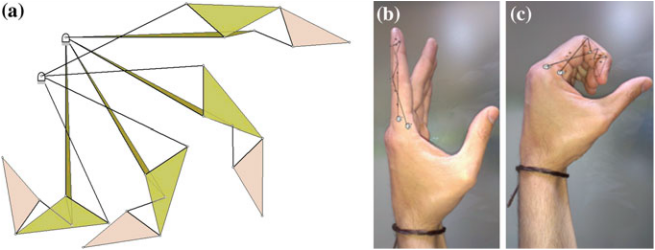
\includegraphics[height=6cm,width=1\textwidth,keepaspectratio]{dimensional_synthesis_exp.png}
        \label{fig:dimensional_synthesis_exp.png}
    \end{figure}
\end{frame}

\begin{frame}[t]{Structural Synthesis}
\framesubtitle{2 questions, which should be answered}
\vspace{-0.6cm}
\begin{figure}[H]
    \begin{minipage}{0.50\textwidth}
        \footnotesize
        \textbf{1) Synthesis of type or Reuleaux synthesis:} What type of mechanism is more suitable? What type of elements will it be made of? Can it be formed by linkages, gears, flexible elements or cams?
        
        Different configurations are developed according to the pre-established requirements. The criteria to value the different characteristics of the mechanism are set.
        \label{reuleaux_synthesis.png}
    \end{minipage}\hfill
    \begin{minipage}{0.48\textwidth}
        \centering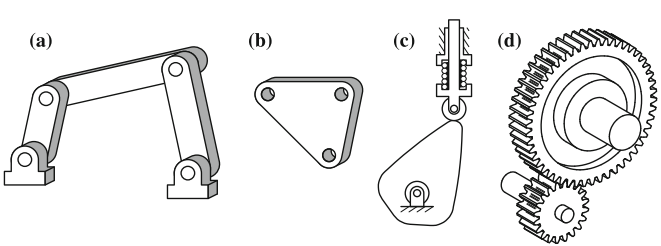
\includegraphics[height=3cm,width=1\textwidth,keepaspectratio]{reuleaux_synthesis.png}
    \end{minipage}
\end{figure}
\vspace{-0.6cm}

\begin{figure}[H]
    \begin{minipage}{0.50\textwidth}
        \footnotesize
        \textbf{2) Synthesis of number or Grübler synthesis:} In the case of a linkage, it determines the number of links and their configuration. 
        \label{grubler_synthesis.png}
    \end{minipage}\hfill
    \begin{minipage}{0.48\textwidth}
        \centering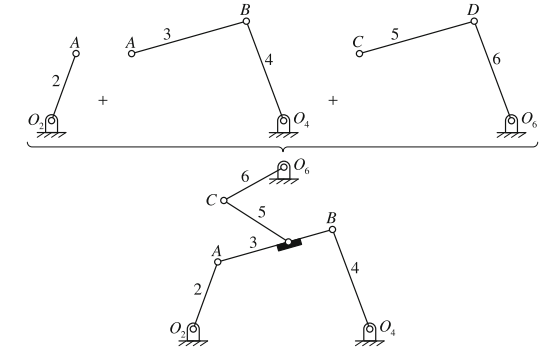
\includegraphics[height=3cm,width=1\textwidth,keepaspectratio]{grubler_synthesis.png}
    \end{minipage}
\end{figure}
\end{frame}

\begin{frame}[t]{Dimensional Synthesis}
\framesubtitle{Functional Generation}
Pre-established conditions refer to the relation between the input and output motions. These are defined by variables $\phi$ and $\psi$, that indentify their positions.
    \begin{figure}[H]
        \centering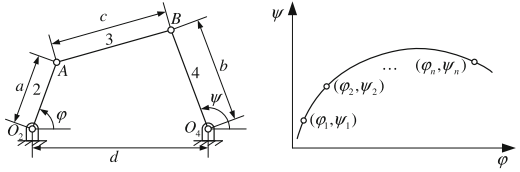
\includegraphics[height=3cm,width=1\textwidth,keepaspectratio]{func_gen1.png}
        % \caption{caption_name}
        \label{fig:func_gen1.png}
    \end{figure}
\end{frame}

\begin{frame}[t]{Dimensional Synthesis}
\framesubtitle{Application}
    \begin{columns}[T,onlytextwidth]
        \begin{column}{0.49\textwidth}
            Function generation can be used to design mechanisms that carry out mathematical operations: addition, differentiation, integration or a combination of them. \smallskip

            The first computers were mechanical devices based on this type of mechanisms.
        \end{column}
        \begin{column}{0.49\textwidth}
            \vspace{-1cm}
            \begin{figure}[H]
                \centering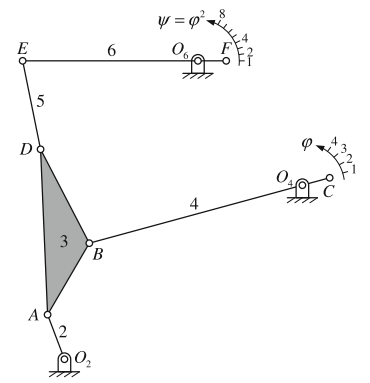
\includegraphics[height=6cm,width=1\textwidth,keepaspectratio]{func_gen2.png}
                \label{fig:func_gen2.png}
            \end{figure}
        \end{column}
    \end{columns}
\end{frame}

\begin{frame}[t]{Dimensional Synthesis}
\framesubtitle{Trajectory Generation}
    \begin{columns}[T,onlytextwidth]
        \begin{column}{0.49\textwidth}
            It studies and provides methods in order to obtain mechanisms in which one of the points describes a given trajectory
        \end{column}
        \begin{column}{0.49\textwidth}
            \vspace{-1cm}
            \begin{figure}[H]
                \centering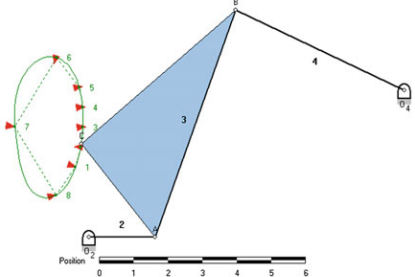
\includegraphics[height=6cm,width=1\textwidth,keepaspectratio]{traj_gen1.png}
                % \caption{caption_name}
                \label{fig:traj_gen1.png}
            \end{figure}
        \end{column}
    \end{columns}
\end{frame}

\begin{frame}[t]{Types of solving methods}
\framesubtitle{}
    \begin{exampleblock}{Graphical}
        These methods are very didactic and help us to understand the problem in an easy way. However, they offer a limited range of possibilities.
    \end{exampleblock}
    
    \begin{exampleblock}{Analytical}
        They solve the problem by means of mathematical equations based on the requirements.
    \end{exampleblock}
    
    \begin{exampleblock}{Optimization-technique-based}
        They can find the optimal solution to the problem by means of the minimization of an objective function and the establishment of a series of restrictions. Different optimization techniques can be used.
    \end{exampleblock}

\end{frame}

\begin{frame}[t]{Reference material}
    \framesubtitle{}
    \begin{enumerate}
        \item \href{https://disk.yandex.ru/i/GCbdbYRq94vbxA}{Synthesis of planar mechanisms (chapter from book)}
        \item \href{https://link.springer.com/book/10.1007/978-3-319-31970-4\#toc}{\textit{"Fundamentals of Machine Theory and Mechanisms" book}}
        \item \href{https://www.geogebra.org/m/SF2rQXEp}{Collection of applets on the Synthesis of Mechanisms (Geogebra)}
        \item \href{https://www.youtube.com/playlist?list=PLH1r3LGlktdvKBfxlcIji4Shf_RrWw8on}{Mechanics of Machinery (MOM) Module 6 Synthesis of Mechanisms (YouTube)}
    \end{enumerate}
\end{frame}



\fbckg{fibeamer/figs/last_page.png}
\frame[plain]{}

\end{document}